\section{Introduction}

Since the creation of Inductive Program Synthesis (IPS) in the 1970s\cite{Kitzelmann2009}, researchers have been striving to create systems capable of generating programs competitively with human intelligence. Modern IPS methods often trace their roots to the fields of machine learning, logic programming, evolutionary computation and others.

The similarities and differences of these methods have been discussed\cite{Kitzelmann2009}, but their performance is rarely compared on problem sets that could provide concrete insight into the capabilities and limitations of each method.

A demonstrative problem set has been compiled that assess an IPS method's ability to work within a range of levels of abstraction\cite{Gaunt2016}, manipulate a variety of data types, produce complex control structures and produce an arbitrary number of outputs of various forms\cite{Helmuth2015b}.

\todo{We need to define exactly what we mean by ``solution'', since it's different
	for GP and, e.g., MagicHaskeller. GP won't \emph{always} find a solution.}

This investigation is exclusively considering a methods ability to find solutions. Other measures, such as runtime or hardware models, are not discussed. In order to asses if a method can find solutions to a problem, the problem must first be phrased, in its entirety, to the method. This is not always possible.

The conclusions drawn from this comparison will speak to the flexibility of each considered method, as well as each method's success rate.

\section{Current State of the Art}



\subsection{Flash Fill}

Flash Fill is a program synthesis technique found in Microsoft Excel \cite{Gulwani2011}. It was designed to help non-programmers perform repetitive tasks that would otherwise require them to write Excel macro programs. It specializes in tasks that require string manipulations. 

To test Flash Fills performance with our problem set, an Excel spreadsheet with one column per input and one column per output was created for each problem. Each spreadsheet included training data, which had both the input and output column populated, and unseen testing data, which left the output column cells empty.

Flash Fill is deterministic and analytic, thus it was only run once per problem on a single data set.

Excel does not include a native vector or list data structure, and it is not clear what the best way to phrase problems that require vectors to Flash Fill. A string representation of vectors was attempted for some problems, as well as putting each item from each vector in a separate cell. These approaches occasionally yielded results, but it is not clear what the optimal usage is.

\subsection{MagicHaskeller}

\todo[inline]{Write me!}

\subsection{TerpreT}

TerpreT is a recently developed, probabilistic programming language that is designed for inductive program synthesis. Problems are specified in the TerpreT language, which is then translated into four different back-end inference algorithms: Forward Marginals Gradient Descent (FMGD), Integer Linear Programming (ILP), Satisfiability modulo theories (SMT) and SKETCH.

The TerpreT system attempts to solve IPS problems using these back-end algorithms and returns source code containing the successful parameters found by the successful back-end algorithm, if one is present.

Note that there is currently no publicly available implementation of TerpreT and thus only results on benchmark problems provided by the original authors could be obtained. It would be extremely valuable to compare TerpreT's performance on the rest of our problem set once an implementation becomes available.


\subsection{Genetic Programming}

Soon after the rise of evolutionary computations, John R. Koza recognized that evolution could be used for more than optimizing a fixed structure of values. In the 1990s, Koza built upon genetic algorithms in such a way that produced executable programs. This technique, named Genetic Programming (GP), is considered inductive program synthesis because it uses input-output examples (refered to as test cases in the field of GP) to evolve a function. In fact, IPS was one of the origional motivations for creating the field of GP\cite{Koza1992}. 

Genetic Programming works by generating a initial population of random programs. Traditionally these programs are represented as trees where non-leaf nodes each denote a function. The children of each non-leaf node are used as the arguments to their parents. Leaf nodes denote terminal values that could be either a constant or input value. This initial population of random programs then follows the cycle in Figure \ref{fig:evo}  until a solution is found or the run is considered a failure.

\begin{figure}[t]
\centering
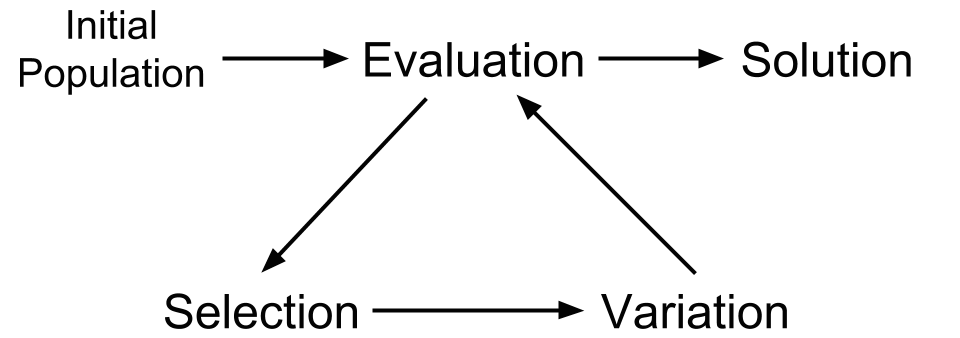
\includegraphics[width=0.25\textwidth]{res/EvolutionCycle}
\caption{Evolutionary Computation process.}
\label{fig:evo}
\end{figure}

\subsubsection{PushGP}

\todo[inline]{Write me!}
\todo[inline]{Why PushGP for IPS?}

\section{Problems}
\subsection{Basic Execution Models Problems}
The first set of problems were taken from \cite{Gaunt2016} and were intended to demonstrate TerpreT's ability to synthesis programs in a variety of execution models that span multiple levels of abstraction. These execution models are: Turing Machine, Boolean Circuits, Basic Block, and Assembly Language. 

As stated by \cite{Gaunt2016}, the problems in this set progress from more abstract execution models towards models which resemble assembly languages. This makes these problems demonstrative of how a system performs across a variety of low-level domains. 
 
The problems in this set are describes below:

\subsubsection{Invert}

Given a binary string (binary tape), invert all the bits.

\subsubsection{Prepend Zero}

Insert a $0$ in the first index of a binary string and shift all other bits to the right.

\subsubsection{Binary Decrement}

Given an input binary string equal to a positive decimal number, return a binary string equal to the input number decremented by one.

\subsubsection{2-bit Controlled Shift Register}

Given input bit ($r_1$, $r_2$, $r_3$), return the same bits, except swap the order of $r_2$ and $r_1$ if $r_1 == 1$.

\subsubsection{Full Adder}

Given a carry bit, $c_{in}$, and two argument bits, $a$ and $b$ , output a sum bit, $s$, and carry bit, $c_{out}$, such that  $s + 2c_{out} = c_{in} + a_1 + b_1$.

\subsubsection{2-bit Adder}

Given input bits $a_1$, $a_2$, $b_1$, and $b_2$, output $s_1$, $s_2$, and $c_{out}$ such that  $s_1 + 2s_2 + 4c_{out} = a_1 + b_1 + 2(a_2 + b_2)$.

\subsubsection{Access}

Given an input array, $V$, and a positive integer, $i$, return $V_i$. Assume $0 < i < |A|$.

\subsubsection{Decrement}

Given an input array, $V$ return a new array, $U$ such that $U_i = V_i - 1$.


\subsection{General Program Synthesis Benchmark Suite}
The second set of problems used in this comparison was proposed by \cite{Helmuth2015b} in order to provide the field of Genetic Programming with a set of non-trivial benchmark problems.

This problems set included problems that deal with multiple data types, including strings, numbers, boolean and vectors. There are also multiple problems in the set that require multiple output values, or printing certain values to the screen.

Given that the Basic Execution Models problem set is designed to test a systems ability to perform in low-level domains (binary circuits, assembly language, etc), the General Program Synthesis Benchmark Suite is an excellent addition, given that the problems' origins assume a much higher-level implementation (ie. java).

%\subsubsection{Number IO}
%\subsubsection{Small or Large}
%\subsubsection{For Loop Index}
%\subsubsection{Compare String Lengths}
%\subsubsection{Double Letters}
%\subsubsection{Collatz Numbers}
%\subsubsection{Replace Space with Newline}
%\subsubsection{String Differences}
%\subsubsection{Even Squares}
%\subsubsection{Wallis Pi}
%\subsubsection{String Lengths Backwards}
%\subsubsection{Last Index of Zero}
%\subsubsection{Vector Average}
%\subsubsection{Count Odds}
%\subsubsection{Mirror Image}
%\subsubsection{Super Anagrams}
%\subsubsection{Sum of Squares}
%\subsubsection{Vectors Summed}
%\subsubsection{X-Word Lines}
%\subsubsection{Pig Latin}
%\subsubsection{Negative To Zero}
%\subsubsection{Scrabble Score}
%\subsubsection{Word Stats}
%\subsubsection{Checksum}
%\subsubsection{Digits}
%\subsubsection{Grade}
%\subsubsection{Median}
%\subsubsection{Smallest}
%\subsubsection{Syllables}

\section{Results}

\begin{figure}
\begin{tabular}{ r | c c c c }
	& TerpreT & Flash Fill & MH & PushGP \\
	\hline
	Invert & \checkmark &  & \checkmark & \checkmark \\
	Prepend Zero & \checkmark & \checkmark & \checkmark & \checkmark \\
	Binary Decrement & \checkmark &  &  &  \\
	2BCSR & \checkmark &  &  & \checkmark \\
	Full Adder & \checkmark &  &  & \checkmark \\
	2 Bit Adder & \checkmark &  &  &  \\
	Access & \checkmark &  & \checkmark & \checkmark \\
	Decrement & \checkmark &  & \checkmark & \checkmark \\
\end{tabular}
\caption{Results of all 4 systems on the Basic Execution Models problems from \cite{Gaunt2016}. A check denotes the system could find a solution.}
\label{fig:results1}
\end{figure}

\begin{figure}
\begin{tabular}{ r | c c c c }
	& Flash Fill & MH & PushGP \\
	\hline
	Number IO &  & \checkmark & \checkmark  \\
	Small Or Large &  &  & \checkmark  \\
	For Loop Index & ? &  & \checkmark  \\
	Compare String Lengths & ? &  & \checkmark  \\
	Double Letters & ? &  & \checkmark  \\
	Collatz Numbers & ? &  &   \\
	Replace Space with Newline & ? &  & \checkmark  \\
	String Differences & ? &  &   \\
	Even Squares & ? &  & \checkmark  \\
	Wallis Pi & ? &  &   \\
	String Lengths Backwards & ? & \checkmark  & \checkmark \\
	Last Index of Zero & ? &  & \checkmark  \\
	Vector Average & ? & \checkmark & \checkmark  \\
	Count Odds & ? &  & \checkmark  \\
	Mirror Image & ? &  & \checkmark  \\
	Super Anagrams & ? &  & \checkmark  \\
	Sum of Squares & ? &  & \checkmark  \\
	Vectors Summed & ? & \checkmark & \checkmark  \\
	X-Word Lines & ? &  & \checkmark  \\
	Pig Latin & ? &  & \checkmark  \\
	Negative To Zero & ? & \checkmark & \checkmark  \\
	Scrabble Score & ? &  & \checkmark  \\
	Word Stats & ? &  &   \\
	Checksum & ? &  &   \\
	Digits & ? &  & \checkmark  \\
	Grade & ? &  & \checkmark  \\
	Median & ? &  & \checkmark  \\
	Smallest & ? & \checkmark & \checkmark  \\
	Syllables & ? &  & \checkmark  \\
\end{tabular}
\caption{Results of all 4 systems on the Basic Execution Models problems from \cite{Gaunt2016}. A check denotes the system could find a solution.}
\label{fig:results2}
\end{figure}

\section{Conclusion}


\section{Outline}

\begin{outline}
 \1 Introduction
   \2 Motivation for Software synthesis
   \2 Historical connection to GP
 \1 State of the art
  \2 Flash Fill
  \2 Magic Haskeller
  \2 TerpreT
  \2 GP
   \3 Push GP is the right way to do software synthesis
 \1 Comparisons
  \2 Problems from TerpreT paper
  \2 Problems from Software Synthesis Benchmark paper
 \1 Results
  \2 Which problems were able to be posed to each method
  \2 Which methods were able to find solutions to each problem
 \1 Conclusion
\end{outline}

\subsection{Things to mention somewhere}
\begin{itemize}
 \item Differences in runtime
 \item FashFill and MagicHaskeller come up with same think every time. GP might not.
 \item MagicHaskeller being hosted on web has pros (crowdsources training) and cons (difficult to integrate in other systesm, large usages could bring it down for everyone)
 \item TerpreT is not available as an open source project yet.
 \item Some systems designed with program readability in mind, others not.
 \item We used boolean vectors as binary tape from TerpreT problems.
 \item We considered the Access problem and the List-k problem to be synonymous in most contexts.
\end{itemize}